\documentclass[12pt]{article}
\usepackage{amsmath, amssymb, amsfonts, bm, graphicx, geometry, tabularx, booktabs, float, enumitem, cancel}
\geometry{margin=1in}

\title{}
\date{}
\author{}

% Uppercase Volume with thicker, higher line
\newcommand{\vol}{\mathord{\text{\ooalign{\hidewidth $V$\hidewidth\cr\kern-0.5pt\raisebox{0.8ex}{\rule[0pt]{1em}{0.5pt}}}}}}

% Lowercase Volume with built-in shifts
\newcommand{\svol}{%
  \mathord{\text{\ooalign{%
    \hfil$v$\hfil\cr
    \hfil\rule[0.6ex]{0.8em}{0.5pt}\hfil
  }}}%
}

\begin{document}

\section*{6-17}
\vspace{-2em}
\begin{center}
    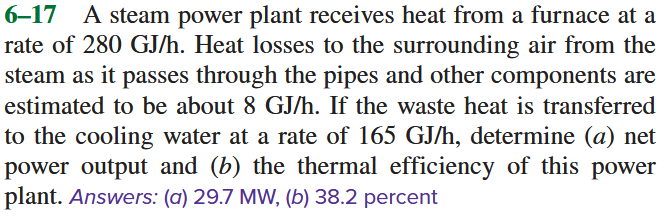
\includegraphics[width=0.7\textwidth]{6-17.png}
\end{center}
\begin{minipage}[t]{0.5\textwidth}
    Given:
\begin{itemize}
    \item $\dot{Q}_{\text{H}} = 280$ GJ/hr
    \item $\dot{Q}_{\text{loss}} = 8$ GJ/hr
    \item $\dot{Q}_\text{L} = 165$ GJ/hr
\end{itemize}
\end{minipage}
\hfill
\begin{minipage}[t]{0.5\textwidth}
Find:
\begin{itemize}
    \item $\dot{W}_{\text{net}}$
    \item $\eta_{\text{th}}$
\end{itemize}
\end{minipage}\\\\
This is a \textbf{heat engine} since it takes in heat to produce work. We use a first law analysis (closed system) to find the net work output:
\[\Delta U = \sum Q - \sum W \implies \dot{U} = \sum \dot{Q} - \sum \dot{W}\]
Since the system is a cycle, $\Delta U = 0 \implies \dot{U} = 0$, so we have
\[(\dot{Q}_H - \dot{Q}_{\text{loss}} - \dot{Q}_L) - \dot{W}_{\text{net}} = 0\]
\[\implies \dot{W}_{\text{net}} = \dot{Q}_H - \dot{Q}_{\text{loss}} - \dot{Q}_L = [280 - 8 - 165\,\text{GJ/hr}] = 107 \text{ GJ/hr}\]
Converting to MW:
\[\dot{W}_{\text{net}} = [107 \text{ GJ/hr}] \cdot \left[\frac{1\,\text{hr}}{3600\,\text{s}}\right] \cdot \left[\frac{10^3\,\text{MJ}}{1\,\text{GJ}}\right] = 29.72 \,\text{MJ/s} = \boxed{29.72 \,\text{MW}}\]
The thermal efficiency is the ratio of net work output to heat input:
\[\eta_{\text{th}} = \frac{\dot{W}_{\text{net}}}{\dot{Q}_H} = \frac{[107 \text{ GJ/hr}]}{[280\,\text{GJ/hr}]} = \boxed{0.3821}\]

\section*{6-57}
\vspace{-2em}
\begin{center}
    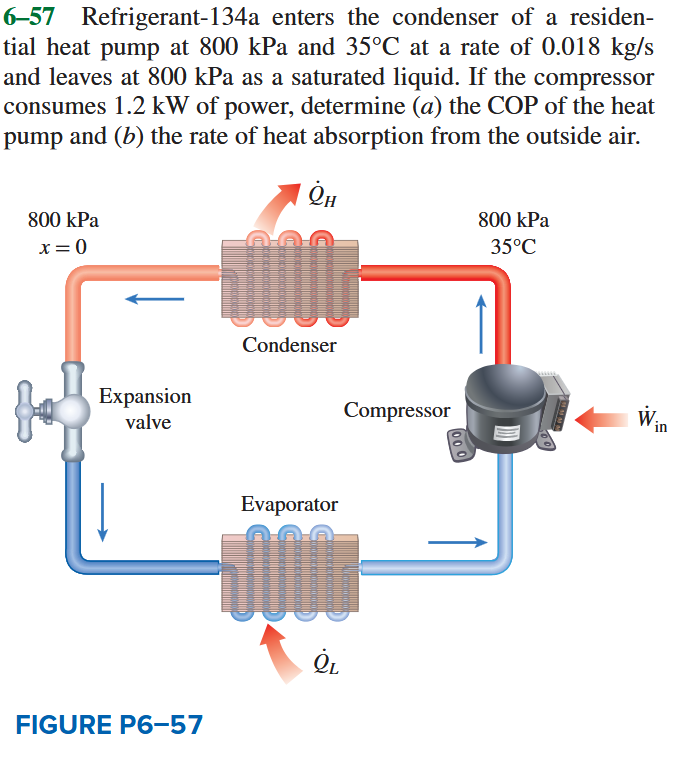
\includegraphics[width=0.7\textwidth]{6-57.png}
\end{center}
\begin{minipage}[t]{0.5\textwidth}
Given:
\begin{itemize}
    \item State 1 (R-134a entering condenser):
    \begin{itemize}
        \item $P_1 = 800$ kPa
        \item $T_1 = 35^\circ$C
        \item $\dot{m}_1 = 0.018$ kg/s
    \end{itemize}
    \item State 2 (leaving condenser):
    \begin{itemize}
        \item $P_2 = 800$ kPa
        \item Saturated liquid $\implies x_2 = 0$
    \end{itemize}
    \item $\dot{W}_\text{in}=1.2$ kW
\end{itemize}
\end{minipage}
\hfill
\begin{minipage}[t]{0.5\textwidth}
Find:
\begin{itemize}
\item  Coefficient of performance (COP) of the \textit{heat pump} (using work to heat the surroundings)
\item Rate of heat absorption from the surroundings ($\dot{Q}_\text{L}$)
\end{itemize}
\end{minipage}\\\\
\textbf{(a)} First, using a first law analysis on the compressor (open system) to determine $\dot{Q}_H$:
\[\frac{dE}{dt} = \dot{Q} - \dot{W} + \sum\dot{m}_i \left[h_i+\frac{1}{2}v_i^2 + gz_i\right] - \sum\dot{m}_e \left[h_e+\frac{1}{2}v_e^2 + gz_e\right]\]
\newpage\noindent
We can simplify the first law equation as follows:
\begin{itemize}
\item No work is done by the system ($\dot{W}=0$)
\item Steady state ($\frac{dE}{dt}=0$)
\item Neglect potential energy changes ($g z_i \approx g z_e$)
\item Neglect kinetic energy changes ($\frac{1}{2}v_i^2 \approx \frac{1}{2}v_e^2$)
\item By conservation of mass, $\dot{m}_1 = \dot{m}_2$
\end{itemize}
Thus, the first law simplifies to:
\[0 = \dot{Q} + \dot{m}_1h_1 -\dot{m}_2h_2\]
\[\implies \dot{Q}_H = \dot{m}_1(h_2 - h_1)\]
From the property tables for R-134a, we have
\begin{itemize}
    \item State 1: (Superheated vapor) $T_1 > T_{\text{sat}}$ at $P_1=800$ kPa. Thus, linear interpolation from the superheated vapor table using values at
    \begin{itemize}
        \item $T=T_{\text{sat}}=31.31^\circ$C: $h_{\text{sat}}=267.34$ kJ/kg
        \item $T=40^\circ$C: $h=276.46$ kJ/kg
    \end{itemize}
    \[h-h_{\text{sat}} = \frac{h_{40} - h_{\text{sat}}}{T_{40} - T_{\text{sat}}} (T - T_{\text{sat}})\]
    \[h=267.34 +1.049(T - 31.31)\quad\implies h_1 =271.212 \,\text{kJ/kg}\]
    \item State 2 (saturated liquid): $h_2 = h_f = 95.48$ kJ/kg
\end{itemize}
Thus, we have
\[\dot{Q}_H = [0.018 \text{ kg/s}] \cdot [95.48 - 271.212 \text{ kJ/kg}] = -3.163 \text{ kW}\]
The negative sign confirms that heat is leaving the system. For the COP, we will use the magnitude of $\dot{Q}_H$:
\[\beta_{\text{HP}} = \frac{|\dot{Q}_H|}{\dot{W}_{\text{in}}} = \frac{[3.163\,\text{kW}]}{[1.2\,\text{kW}]} = \boxed{2.635}\]
\textbf{(b)} Applying the first law to the entire heat pump cycle (closed system):
\[\Delta U = \sum Q - \sum W \implies \dot{U} = \sum \dot{Q} - \sum \dot{W}\]
Since the system is a cycle, $\Delta U = 0 \implies \dot{U} = 0$, so we have:
\[(\dot{Q}_H - \dot{Q}_L) - \dot{W}_{\text{in}} = 0\]
Again, using magnitudes for the heat transfer rates (since direction is already accounted for):
\[\implies \dot{Q}_L = \dot{Q}_H - \dot{W}_{\text{in}} = [3.163 - 1.2 \text{ kW}] = \boxed{1.963 \text{ kW}}\]

\section*{6-84E}
\vspace{-2em}
\begin{center}
    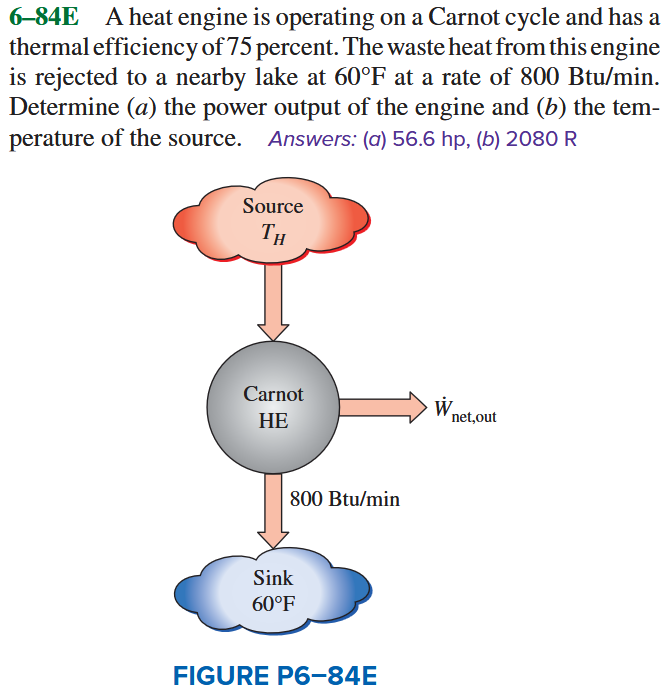
\includegraphics[width=0.7\textwidth]{6-84E.png}
\end{center}
\begin{minipage}[t]{0.5\textwidth}
Given:
\begin{itemize}
    \item $\eta_{\text{th}} = 0.75$
    \item $\dot{Q}_L = 800$ Btu/min
    \item $T_L = 60^\circ$F
\end{itemize}
\end{minipage}
\hfill
\begin{minipage}[t]{0.5\textwidth}
Find:
\begin{itemize}
\item $\dot{W}_{\text{net,out}}$
\item $T_H$
\end{itemize}
\end{minipage}\\\\
Given that this is a \textit{carnot heat engine} (reversible and takes in heat to generate work), we can use the following relationships:
\[\eta_\text{carnot} = \frac{\dot{W}_\text{net,out}}{\dot{Q}_H}=1 - \frac{\dot{Q}_L}{\dot{Q}_H} = 1 - \frac{T_L}{T_H}\]
\underline{Note:} The heat terms may be expressed either as total heat ($Q$) or heat transfer rates ($\dot{Q}$), since the time dependence cancels in the efficiency ratio.\\\\
\textbf{(a)} By definition of thermal efficiency, we can find $\dot{Q}_H$:
\[\eta_{\text{th}} = 1 - \frac{\dot{Q}_L}{\dot{Q}_H}\]
\[\implies \dot{Q}_H = \frac{\dot{Q}_L}{1 - \eta_{\text{th}}} = \frac{[800\,\text{Btu/min}]}{1 - 0.75} = 3200 \text{ Btu/min}\]
Now we can find the net work output:
\[\eta_{\text{th}} = \frac{\dot{W}_{\text{net,out}}}{\dot{Q}_H} \implies \dot{W}_{\text{net,out}} = \eta_{\text{th}} \cdot \dot{Q}_H\]
\[\dot{W}_{\text{net,out}} = 0.75 \cdot [3200 \text{ Btu/min}] = 2400 \text{ Btu/min}\]
Converting to hp:
\[\dot{W}_{\text{net,out}} = [2400 \text{ Btu/min}] \cdot \left[\frac{778.169\,\text{ft}\cdot\text{lbf}}{1\,\text{Btu}}\right]\cdot\left[\frac{1\,\text{min}}{60\,\text{s}}\right]\cdot\left[\frac{1\,\text{hp}}{550\,\text{ft}\cdot\text{lbf/s}}\right] = \boxed{56.59\,\text{hp}}\]
\textbf{(b)} Using the Carnot efficiency relationship:
\[\eta_\text{carnot} = 1 - \frac{T_L}{T_H}\]
\[\implies T_H = \frac{T_L}{1 - \eta_\text{carnot}} = \frac{[60 + 459.67]\,\text{R}}{1 - 0.75} = \boxed{2078.68 \text{ R}}\]

\section*{6-103}
\vspace{-2em}
\begin{center}
    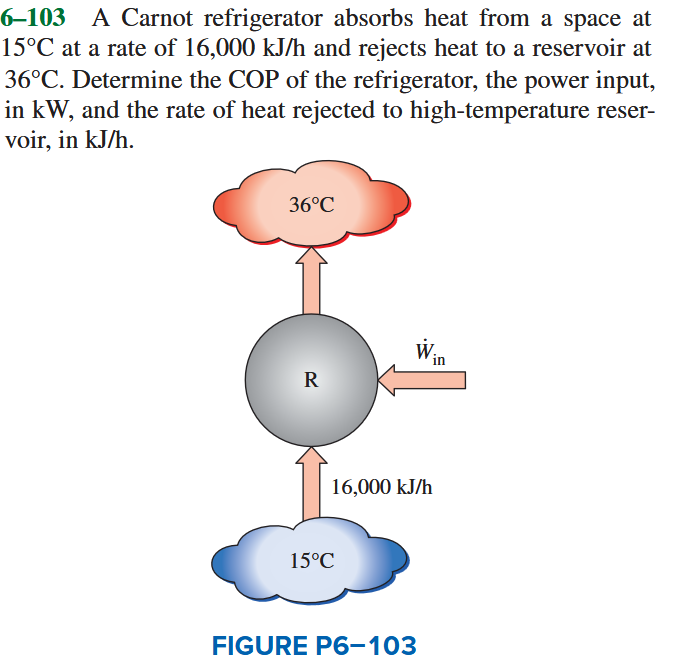
\includegraphics[width=0.7\textwidth]{6-103.png}
\end{center}
\begin{minipage}[t]{0.5\textwidth}
Given:
\begin{itemize}
    \item $T_L = 15^\circ$C
    \item $\dot{Q}_L = 16,000$ kJ/hr
    \item $T_H = 36^\circ$C
\end{itemize}
\end{minipage}
\hfill
\begin{minipage}[t]{0.5\textwidth}
Find:
\begin{itemize}
\item $\beta_\text{ref}$
\item $\dot{W}_\text{in}$ [kW]
\item $\dot{Q}_H$ [kJ/hr]
\end{itemize}
\end{minipage}\\\\
First law for a closed system (cycle):
\[\dot{U} = \sum \dot{Q} - \sum \dot{W} \implies 0 = (\dot{Q}_L - \dot{Q}_H) - (-\dot{W}_\text{in}) \implies\dot{W}_\text{in} = \dot{Q}_H - \dot{Q}_L \]
\underline{Note:} Sign conventions! Work is negative since it's entering and heat is positive when it's entering the system.\\\\
For a \textit{carnot refrigerator} (reversible and uses work to absorb heat from the surroundings), we can use the following relationships:
\[\beta_\text{carnot ref} = \frac{\dot{Q}_L}{\dot{W}_\text{in}} = \frac{\dot{Q}_L}{\dot{Q}_H - \dot{Q}_L}= \frac{T_L}{T_H - T_L}\]
\textbf{(a)} Using the Carnot refrigerator relationship:
\[T_L = 15 + 273.15 = 288.15 \text{ K},\quad T_H = 36 + 273.15 = 309.15 \text{ K}\]
\[\beta_\text{ref} = \frac{T_L}{T_H - T_L} = \frac{288.15}{309.15 - 288.15} = \boxed{13.72}\]
\underline{Note:} CONVERT TO ABSOLUTE TEMPERATURES!\\\\
\textbf{(b)} Using relationship:
\[\beta_\text{carnot ref} = \frac{\dot{Q}_L}{\dot{W}_\text{in}} \implies \dot{W}_\text{in} = \frac{\dot{Q}_L}{\beta_\text{carnot ref}}\]
\[\dot{W}_\text{in} = \frac{[16,000 \text{ kJ/hr}]}{13.72} = 1166.18 \text{ kJ/hr}\]
Converting to kW:
\[\dot{W}_\text{in} = [1166.18 \text{ kJ/hr}] \cdot \left[\frac{1\,\text{hr}}{3600\,\text{s}}\right] = \boxed{0.323 \text{ kW}}\]
\textbf{(c)} Using the first law relationship:
\[\dot{Q}_H = \dot{Q}_L + \dot{W}_\text{in} = [16000 + 1166.18\,\text{kJ/hr}] = \boxed{17166.18 \text{ kJ/hr}}\]

\newpage
\section*{6-106}
\vspace{-2em}
\begin{center}
    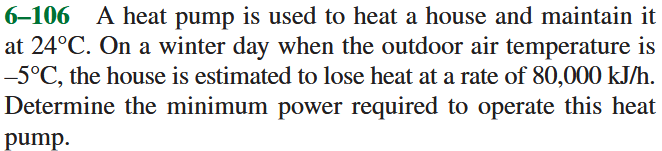
\includegraphics[width=0.7\textwidth]{6-106.png}
\end{center}
\begin{minipage}[t]{0.5\textwidth}
Given:
\begin{itemize}
    \item $T_L = -5^\circ$C = 268.15 K
    \item $T_H = 24^\circ$C = 297.15 K
    \item $\dot{Q}_\text{loss} = 80,000$ kJ/hr
\end{itemize}
\end{minipage}
\hfill
\begin{minipage}[t]{0.5\textwidth}
Find:
\begin{itemize}
\item \textit{Minimum} power required to operate the heat pump
\end{itemize}
\end{minipage}\\\\
A heat pump uses work to transfer heat from a low temperature reservoir to a high temperature reservoir. Since the house stays at a constant temperature, we can see that 
\[\dot{Q}_H = \dot{Q}_\text{loss}\]
Additionally, it asks for the \textit{minimum} power required, and the most efficient process is the carnot process, so we can use the Carnot heat pump relationship:
\[\beta_\text{carnot HP} = \frac{\dot{Q}_H}{\dot{W}_\text{in}} = \frac{T_H}{T_H - T_L}\]
\[\implies \beta_\text{carnot HP} = \frac{[297.15\,\text{K}]}{[297.15 - 268.15\,\text{K}]} = 10.24\]
\[\dot{W}_\text{in} = \frac{\dot{Q}_H}{\beta_\text{carnot HP}} = \frac{\dot{Q}_\text{loss}}{\beta_\text{carnot HP}}\]
\[\implies \dot{W}_\text{in} = \frac{[80,000\,\text{kJ/hr}]}{10.24} = 7812.5\,\text{kJ/hr}\]
Converting to kW:
\[\dot{W}_\text{in} = [7812.5 \text{ kJ/hr}] \cdot \left[\frac{1\,\text{hr}}{3600\,\text{s}}\right] = \boxed{2.17 \text{ kW}}\]
\newpage
\section*{6-135}
\vspace{-2em}
\begin{center}
    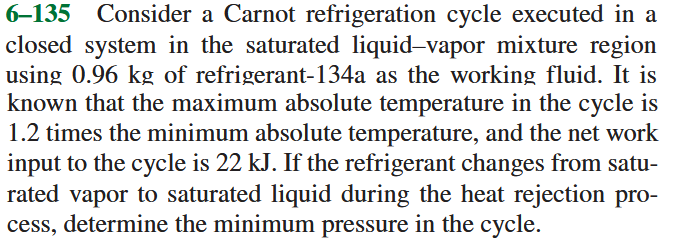
\includegraphics[width=0.7\textwidth]{6-135.png}
\end{center}
For saturated mixtures, pressure and temperature are always related. Additionally, as temperature increases, so does the saturation pressure. Since the R-134a remains as a saturated mixture throughout the cycle, the \textit{minimum} pressure in the cycle MUST be the saturation pressure at the lowest temperature in the cycle. This is at the evaporator, where hot R-134a is cooled to $T_L$.\\\\
We are also told that the R-134a changes phases from saturated vapor to saturated liquid at the condenser, so we can use this to find $Q_H$ (heat rejected as a result of phase change).
\begin{center}
    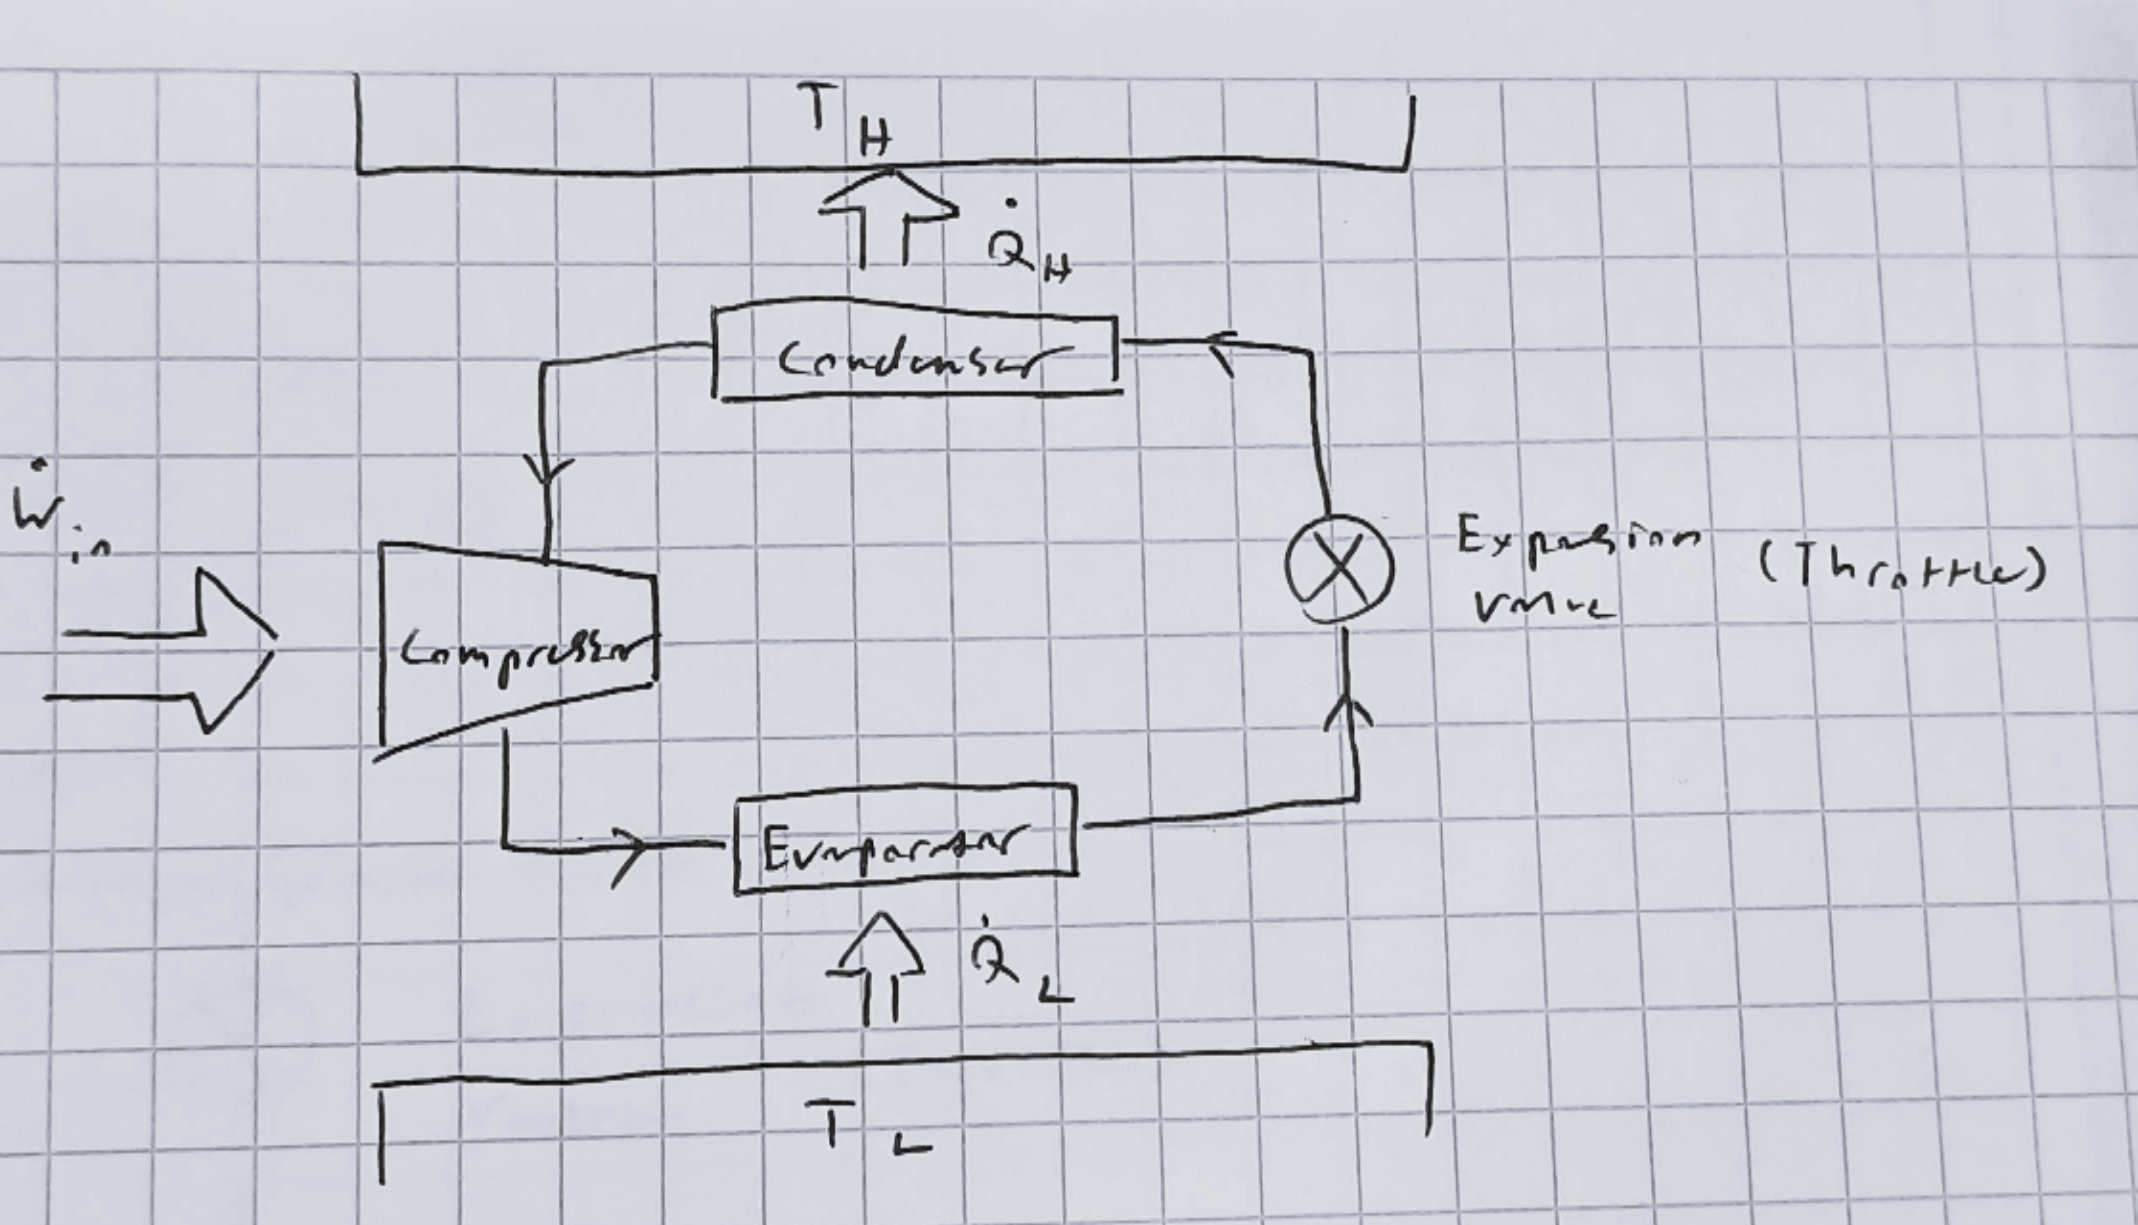
\includegraphics[width=0.7\textwidth]{6-135_1.jpg}
\end{center}
\underline{Note:} Even though the R-134a needs to be colder than $T_L$ to facilitate heat transfer, in an \textit{ideal} reversible cycle, the R-134a is at the same temperature as the surroundings during heat transfer. Thus, we can use $T_L$ to find the saturation pressure at the evaporator.\\\\
\begin{minipage}[t]{0.5\textwidth}
Given:
\begin{itemize}
    \item $m= 0.96$ kg
    \item $T_L$
    \item $T_H = 1.2T_L$
    \item $W_\text{net, in} = 22$ kJ
\end{itemize}
\end{minipage}
\hfill
\begin{minipage}[t]{0.5\textwidth}
Find:
\begin{itemize}
\item \textit{Minimum} pressure in the cycle
\end{itemize}
\end{minipage}
\newpage\noindent
\textbf{(a)} For a carnot refrigerator, we can use the following relationships:
\[\beta_\text{carnot ref} = \frac{{Q}_L}{{W}_\text{in}} = \frac{{Q}_L}{{Q}_H - {Q}_L}= \frac{T_L}{T_H - T_L}\]
\[\implies \beta_\text{carnot ref} = \frac{T_L}{1.2T_L - T_L} = \frac{T_L}{0.2T_L} = 5\]
\[\implies {Q}_L = 5 \cdot {W}_\text{in} = 5 \cdot [22 \text{ kJ}] = 110 \text{ kJ}\]
Now we need to find $Q_H$ to determine $T_H$. Using a first law analysis on the entire cycle (closed system):
\[W + Q_L = Q_H\]
\[\implies Q_H = W + Q_L = 22 \text{ kJ} + 110 \text{ kJ} = 132 \text{ kJ}\]
\textbf{(b)} We can relate $Q_H$ to the enthalpy change during the phase change at the condenser in order to find $T_H$. Using a first law analysis on the condenser (open system):
\[\frac{dE}{dt} = \dot{Q} - \dot{W} + \sum\dot{m}_i \left[h_i+\frac{1}{2}v_i^2 + gz_i\right] - \sum\dot{m}_e \left[h_e+\frac{1}{2}v_e^2 + gz_e\right]\]
\begin{itemize}
\item No work is done by the system ($\dot{W}=0$)
\item Steady state ($\frac{dE}{dt}=0$)
\item Neglect potential energy changes ($g z_i \approx g z_e$)
\item Neglect kinetic energy changes ($\frac{1}{2}v_i^2 \approx \frac{1}{2}v_e^2$)
\item By conservation of mass, $\dot{m}_1 = \dot{m}_2$
\end{itemize}
Thus, the first law simplifies to:
\[0 = \dot{Q} + \dot{m}_1h_1 -\dot{m}_2h_2\]
\[\implies \dot{Q}_H = \dot{m}_1(h_2 - h_1)\]
Integrating over time:
\[Q_H = m(h_2 - h_1)\]
We know that the R-134a changes phases from saturated vapor to saturated liquid at the condenser, so
\[h_2 = h_{f @ T_H},\quad h_1 = h_{g@ T_H}\implies h_2-h_1 = h_{fg @ T_H}\]
\[\implies h_{fg @ T_H} =\frac{Q_H}{m} = \frac{[132 \text{ kJ}]}{[0.96 \text{ kg}]} = 137.5 \text{ kJ/kg}\]
Finding the associated saturation temperature for this value of $h_{fg}$ from the R-134a tables via linear interpolation using values at:
\begin{itemize}
\item $T=60^\circ$C: $h_{fg}=139.09$ kJ/kg
\item $T=65^\circ$C: $h_{fg}=132.05$ kJ/kg
\end{itemize}
\[T - T_{60} = \frac{T_{65} - T_{60}}{h_{fg@65} - h_{fg@60}} (h_{fg} - h_{fg@60})\]
\[\implies T = 60 -0.710 (h_{fg} - 139.09) \implies T_H = 61.129^\circ\text{C}\]
\newpage\noindent
Thus, 
\[T_H = 334.279\,\text{K}\]
\textbf{(c)} Using the carnot refrigerator relationship to finally find $T_L$:
\[\beta_\text{carnot ref}  = \frac{T_L}{T_H - T_L}\]
\[\implies T_L = \frac{\beta_\text{carnot ref} \cdot T_H}{1 + \beta_\text{carnot ref}} = \frac{5 \cdot [334.279\text{ K}]}{1 + 5} = 278.57\,\text{K}\]
Convert to Celsius:
\[T_L = 278.57 - 273.15 = 5.415^\circ\text{C}\]
\textbf{(d)} Finally, we just need to find the saturation pressure at $T_L$ to find the minimum pressure in the cycle. Linear interpolation using values at:
\begin{itemize}
\item $T=4^\circ$C: $P_\text{sat}=337.90$ kPa
\item $T=6^\circ$C: $P_\text{sat}=362.23$ kPa
\end{itemize}
\[P - P_{4} = \frac{P_{6} - P_{4}}{T_{6} - T_{4}} (T - T_{4})\]
\[\implies P = 337.90 + 12.165(T - 4) \implies P_{@ T_L} = 350.065\,\text{kPa}\]
\[\implies \boxed{P_\text{min}=P_{@ T_L} = 350.065\,\text{kPa}}\]

\section*{6-159}
\vspace{-2em}
\begin{center}
    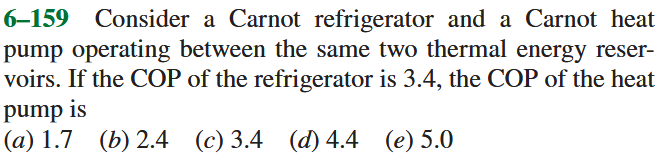
\includegraphics[width=0.7\textwidth]{6-159.png}
\end{center}
Looking at the carnot efficiency relationship for a refrigerator:
\[\beta_\text{carnot ref} = \frac{T_L}{T_H - T_L}=3.4\]
For a heat pump, we have:
\[\beta_\text{carnot heat pump} = \frac{T_H}{T_H - T_L}\]
Since $T_H = (T_H-T_L) + T_L$, we can rewrite the heat pump relationship as:
\[\beta_\text{carnot heat pump} = \frac{(T_H-T_L) + T_L}{T_H - T_L} = 1 + \frac{T_L}{T_H - T_L} = 1 + \beta_\text{carnot ref}\]
\[\implies \beta_\text{carnot heat pump} = 1 + 3.4 = \boxed{4.4\quad\text{(d)}}\]




\end{document}